%%%%%%%%%%%%%%%%%%%%%%%%%%%%%%%%%%%%%%%%%
% Journal Article
% LaTeX Template
% Version 1.3 (9/9/13)
%
% This template has been downloaded from:
% http://www.LaTeXTemplates.com
%
% Original author:
% Frits Wenneker (http://www.howtotex.com)
%
% License:
% CC BY-NC-SA 3.0 (http://creativecommons.org/licenses/by-nc-sa/3.0/)
%
%%%%%%%%%%%%%%%%%%%%%%%%%%%%%%%%%%%%%%%%%

%----------------------------------------------------------------------------------------
%	PACKAGES AND OTHER DOCUMENT CONFIGURATIONS
%----------------------------------------------------------------------------------------

\documentclass[twoside]{article}

\usepackage{lipsum} % Package to generate dummy text throughout this template
\usepackage{graphicx}

\usepackage[sc]{mathpazo} % Use the Palatino font
\usepackage[T1]{fontenc} % Use 8-bit encoding that has 256 glyphs
\linespread{1.05} % Line spacing - Palatino needs more space between lines
\usepackage{microtype} % Slightly tweak font spacing for aesthetics

\usepackage[hmarginratio=1:1,top=32mm,columnsep=20pt]{geometry} % Document margins
\usepackage{multicol} % Used for the two-column layout of the document
\usepackage[hang, small,labelfont=bf,up,textfont=it,up]{caption} % Custom captions under/above floats in tables or figures
\usepackage{booktabs} % Horizontal rules in tables
\usepackage{float} % Required for tables and figures in the multi-column environment - they need to be placed in specific locations with the [H] (e.g. \begin{table}[H])
\usepackage{hyperref} % For hyperlinks in the PDF

\usepackage{lettrine} % The lettrine is the first enlarged letter at the beginning of the text
\usepackage{paralist} % Used for the compactitem environment which makes bullet points with less space between them

\usepackage{abstract} % Allows abstract customization
\renewcommand{\abstractnamefont}{\normalfont\bfseries} % Set the "Abstract" text to bold
\renewcommand{\abstracttextfont}{\normalfont\small\itshape} % Set the abstract itself to small italic text

\usepackage{titlesec} % Allows customization of titles
\renewcommand\thesection{\Roman{section}} % Roman numerals for the sections
\renewcommand\thesubsection{\Roman{subsection}} % Roman numerals for subsections
\titleformat{\section}[block]{\large\scshape\centering}{\thesection.}{1em}{} % Change the look of the section titles
\titleformat{\subsection}[block]{\large}{\thesubsection.}{1em}{} % Change the look of the section titles

\usepackage{fancyhdr} % Headers and footers
\pagestyle{fancy} % All pages have headers and footers
\fancyhead{} % Blank out the default header
\fancyfoot{} % Blank out the default footer
%\fancyhead[C]{Running title $\bullet$ November 2012 $\bullet$ Vol. XXI, No. 1} % Custom header text
\fancyfoot[RO,LE]{\thepage} % Custom footer text

\usepackage{amsmath}
\usepackage{amsmath,amsfonts,amssymb}
%----------------------------------------------------------------------------------------
%	TITLE SECTION
%----------------------------------------------------------------------------------------

\title{\vspace{-15mm}\fontsize{24pt}{10pt}\selectfont\textbf{Speaker Recognition in non-linear signal processing and pattern recognition.}} % Article title

\author{
\large
\textsc{Rune A. Heick, Rasmus S. Reimer \& Nicolai Glud}\\[2mm] % Your name
\normalsize Aarhus University, Department of Engineering \\ % Your institution
\vspace{-5mm}
}
\date{}

%----------------------------------------------------------------------------------------

\begin{document}

\maketitle % Insert title
\thispagestyle{fancy} % All pages have headers and footers
\raggedright

%----------------------------------------------------------------------------------------
%	ABSTRACT
%----------------------------------------------------------------------------------------

\begin{abstract}
The Content of this paper seeks to present the knowledge gained throughout the non-linear signal processing and pattern recognition course from Aarhus University, department of engineering. The paper is split into multiple sections explaining the data used in the paper, the methods used to treat the data and the methods used for categorising the data.
\end{abstract}

%----------------------------------------------------------------------------------------
%	ARTICLE CONTENTS
%----------------------------------------------------------------------------------------

%\begin{multicols}{2} % Two-column layout throughout the main article text

\chapter{Introduction}
Goal

\section{Reading guide}
The report should be seen as four sections, introduction, methods, results and conclusion.\\
The introduction covers the specification of the project by project formulation, system description, requirement specification and project scope.\\
Methods explains the approach to the project and solutions, planning and scheduling, work distribution and project structure.\\
The results covers the result of the project namely what have been made and what have been learned. Most subjects here will be described briefly but further information can be found in the more detailed descriptions in the documentation found on the CD.\\
The conclusion rounds up the project and weighs of expectations and goals.

\section{Glossary and abbreviations}
This section contains all the abbreviations and terms used in this project. The full name will often be written the first time an abbreviation is encountered.\\
The abbreviations and terms are general for the entire project and might not be used in this documents.
\begin{table}[H]
\centering
\begin{tabular}{|p{4cm}|p{7cm}|}
\hline
Term/abbreviation & Definition\\ \hline
PC / computer & General term for a computer / Personal Computer.\\ \hline
\end{tabular}
\end{table}
\section{Data Gathering}
The data used in this project was gathered by recording three different persons reading the same article from the website "www.tv2.dk". The voices was recorded using the software Audacity\footnote{http://sourceforge.net/projects/audacity/} and the Lame mp3 codex\footnote{http://lame.sourceforge.net/}. The data is then imported into matlab using the function \texttt{[data, Fs] = audioread(pathToFile)}. The data is then normalised by removing the mean of the data, and whitening the data. The files are in stereo and both channels are used by appending one channel to the other so to have one long array of data.

\section{Feature Extraction}
The Mel Frequency Cepstral Coefficient method is commonly used to extract features in speech and speaker recognition. The methods provides features that are useful for classifying linguistic content. The basis is that the speech from humans is uniquely filtered by the shape of the vocal tract, tongue, teeth etc\footnote{http://practicalcryptography.com/miscellaneous/machine-learning/guide-mel-frequency-cepstral-coefficients-mfccs/ - retrieved 4 june 2015}. 

MFCCs are found using a series of steps as can be seen in figure \ref{fig:MFCCsteps}.
\begin{figure}[H]
\centering
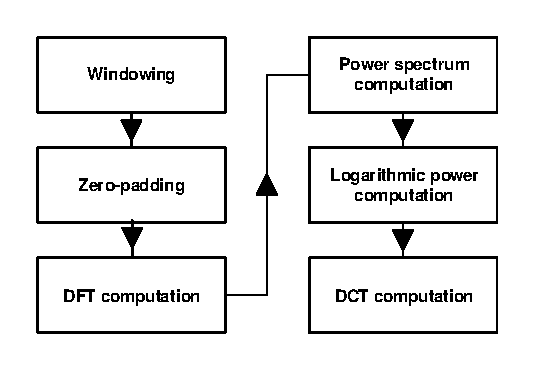
\includegraphics[scale=1]{billeder/MFCCsteps}
\caption{MFCC steps}
\label{fig:MFCCsteps}
\end{figure}
The figure has been derived from the article \cite{Sahidullah2012}. The steps can be described as follows:
\begin{enumerate}
\item Windowing: The speech signal is windows with either a Hamming or Hanning window.
\item Zero-padding: A number of zeros are padded to he windowed speech signal in order to enable fast Fourier transform (FFT).
\item DFT: The windowed speech signal is discrete fourier transformed using a FFT algorithm.
\item Power spectrum: The resulting spectrum is mapped onto the mel scale but utilising a triangular filter bank.
\item Logarithmic power: The power spectrum is converted to logarithmic scale with respect to the mel frequencies.
\item DCT: The logarithmic mel powers are discrete cosine transformed. The MFCCs is the amplitudes of the output spectrum.
\end{enumerate}

In MATLAB this is done using the toolbox, voicebox\footnote{http://www.ee.ic.ac.uk/hp/staff/dmb/voicebox/voicebox.html - retrieved 6 june 2015}. The function for getting the MFCCs is called \texttt{melcepst} and a thorough explaination can be found on the voicebox website\footnote{http://www.ee.ic.ac.uk/hp/staff/dmb/voicebox/doc/voicebox/melcepst.html}. 

In short the function is invoked like this:
\begin{verbatim}
mel = melcepst(data(:,i), Fs(i), 'M0d', nc, p, n, inc);
\end{verbatim}
With \textbf{data} being the signal we want to extract the MFCCs from. 
\textbf{Fs} is the sampling frequency of the signal. 
\textbf{'M0d'} is the mode string and the three characters correspond to Hamming window, include 0'th order cepstral coefficient and include delta coefficients.
\textbf{nc} is the number of cepstral coefficients excluding 0'th coefficient.
\textbf{p} is the number of filters in the filterbank.
\textbf{n} is the length of the frame in the samples.
and lastly \textbf{inc} is the frame increment value.
\fxnote{Possible formatting of this block of text}

In this project the window size is chosen to be 200 milliseconds. The default value for speaker recognition is 150 milliseconds while speech recognition is typically lower than that. The number of cepstral coefficients was chosen to be 30.

The mel output from the function is used for features. The resulting matrix is $M \times N$ with M being number of samples of each MFCC and N being number of MFCCs. For the data used in this project his corresponds to a $2175 \times 62$.


%------------------------------------------------
%!TEX root = ..\Master.tex

\section{Dimensionality Reduction}

e.g. finding projection vectors, choosing number of components, applications.\\

motivation:
data compression
speed up learning algorithm


\subsection{PCA}

Principal component analysis is used for reducing the number of dimensions of a feature space.
It works by projecting the data in the feature space, down to a fewer dimensional feature space by minimizing the squared projection error.
The reduced feature space does not nessecarily share the same features, but new features are found which best retains the variance in the data.

PCA should mainly be used for compressing the data to save memory or reducing running time of learning algorithm.
By reducing the amount of features most machine learning algorithms runs faster.
PCA can also be used to prevent overfitting, but its usually better to use regularization. \\

Figure \ref{fig:pca} shows a 3 dimensional feature space where all the data, within a small margin, lies in a 2 dimensional plane.
PCA is used to find two vectors $u^{(1)}$ and $u^{(2)}$ which spans this 2D plane.

\begin{figure}[H]
\centering
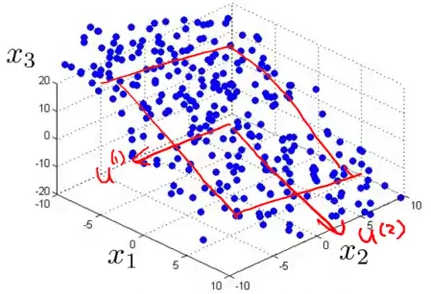
\includegraphics{billeder/pca}
\caption{3D to 2D pca illustration}
\label{fig:pca}
\end{figure}


Preprocessing of the data should be done before doing PCA. \\
Given the training set:
\begin{equation}
x = 
\begin{bmatrix}
x_1 & x_2 & \dots & x_m
\end{bmatrix}
\end{equation}

Ensure that every feature has zero mean by doing mean normalization:
\begin{equation}
\mu_j = \frac{1}{m} \sum^m_{i=1} x_j^{(i)}
\end{equation}
\begin{equation}
x_j = x_j - \mu_j
\end{equation}

Feature scaling can also be done if the features have very different value ranges. TODO \\

After preprocessing the data, we can do PCA on it.\\
We start by computing the covariance matrix $\Sigma$:
\begin{equation}
\Sigma = \frac{1}{m} \sum^n_{i=1} x^{(i)} {x^{(i)}}^T
\end{equation}

The covariance matrix descripes how the different features relates.
When doing feature reduction we want to remove features which has high correlation with other features.
An example could be a feature which descripes a length in cm and another feature descriping the same length in inches.
These features will have very high correlation and one of them can be removed from the feature space without loosing much information. \\

Then we compute the eigenvectors of covariance matrix:
\begin{equation}
U = \begin{bmatrix}
   u^{(1)} & u^{(2)} & \dots & u^{(n)}
 \end{bmatrix}
\in \mathbb{R}^{n \times n}
\end{equation}

The eigenvectors will lay in the directions of most variance in the data.
This is what is shown on Figure \ref{fig:pca}.
The longer the eigenvector, the more variance it descripes.
Therefore we want to keep the longest eigenvectors and remove the shortest eigenvectors.

The eigenvectors are ordered by length in the matrix $U$.
The longest is the first. \\

We select the first $k$ eigenvectors to get the reduced set of eigenvectors:
\begin{equation}
U_{reduce} = \begin{bmatrix}
   u^{(1)} & u^{(2)} & \dots & u^{(k)}
 \end{bmatrix}
\end{equation}

We can now calculate the new feature vectors:
\begin{equation}
z = U_{reduce}^Tx
\end{equation}

We have now reduced the feature space to a $k$ dimensional feature space.
Say we want to retain at least $95\%$ of the variance in the data.
We do this by picking the smallest value of $k$ so that:
\begin{equation}
\frac{\displaystyle\sum^{k}_{i=1} S_{ii}}{\displaystyle\sum^{n}_{i=1} S_{ii}} \geq 0.95
\end{equation}

The matrix $S$ is found by doing singular value decomposition (SVD). The matrix $S$ has the form:
\begin{equation}
S =  
\begin{bmatrix}
S_{11} & 0 & 0 & 0 & 0 \\
0 & S_{22} & 0 & 0 & 0 \\
0 & 0 & S_{33} & 0 & 0 \\
0 & 0 & 0 & \dots & 0 \\
0 & 0 & 0 & 0 & S_{nn} \\
\end{bmatrix}
\end{equation}

In our project we use PCA to reduce our feature space from 64 dimensions down to 40 dimensions.
We do this to increase the speed of our learning algorithms while still retainging almost all of our data ($\geq 99.99\%$) as seen on Figure \ref{fig:pca-on-our-data}.
(TODO: Add axis labels to figure. x = number of features. y = retained variance.)

\begin{figure}[H]
\centering
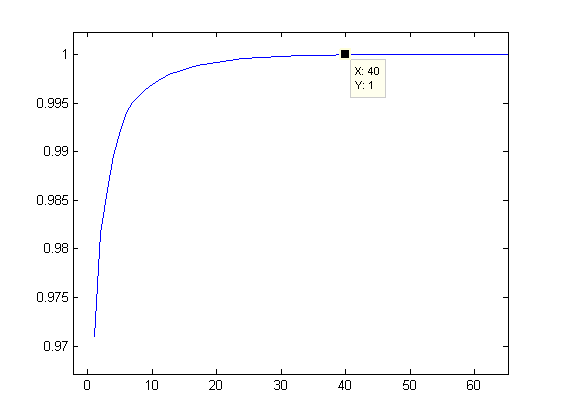
\includegraphics{billeder/pca-on-our-data}
\caption{3D to 2D pca illustration}
\label{fig:pca-on-our-data}
\end{figure}

\subsection{Fisher}

Introtext\\

Math\\

How we use it or why we don't use it\\

Intermediate result\\

%------------------------------------------------

\section{Classifiers}
Classifiers were first know from the world of linear regression. The classifiers found in this section are featured in the non-linear signal processing and pattern recognition course. The section seeks to explain the basis of each of the classifiers along with how we have used them in our project. Intermediate results can be found in the section about the classifiers while the comparison between classifiers can be found in the Results section.
\subsection{Linear Classifier}
The goal of linear classification is to take an input vector with multiple x values and assign it to one of multiple classes K. This can be done with one or more linear decision boundaries. The first way to classify is called the one-vs-one linear classifier. This works for 2 classes as seen in figure \ref{onevsone1}. If multiple clusters of x belonging to more than 2 classes are present we get ambiguous regions as one class might appear to be two different classes. An example of this can be seen in figure \ref{onevsone2}.
\begin{figure}[H]
\centering
\begin{minipage}[b]{0.5\textwidth}
\centering
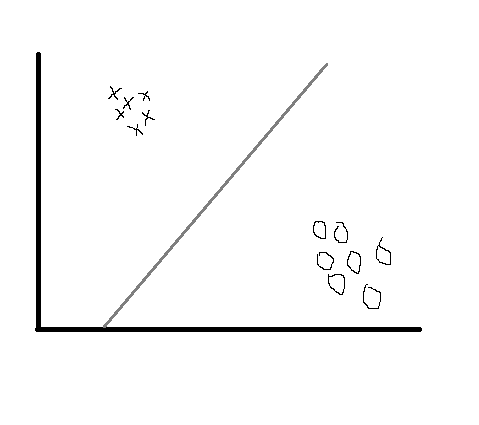
\includegraphics[scale=0.5]{billeder/onevsone1}
\caption{One-vs-one linear classifier for 2 classes}
\label{onevsone1}
\end{minipage}%
\begin{minipage}[b]{0.5\textwidth}
\centering
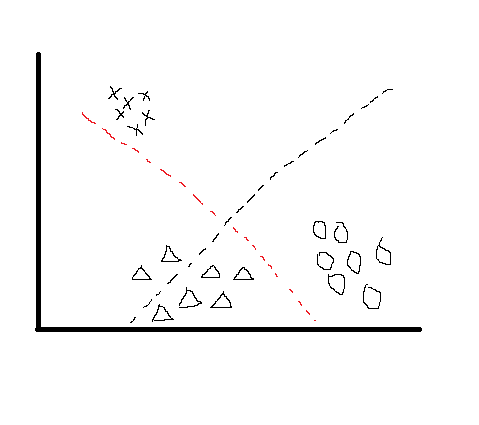
\includegraphics[scale=0.5]{billeder/onevsone2}
\caption{One-vs-one linear classifier for 3 classes}
\label{onevsone2}
\end{minipage}
\end{figure}
Another way to classify  the 3 classes seen in figure \ref{onevsone2} could be to utilise 1-of-k classification. This can be seen in figure \ref{oneofk1}. The 1-of-k classifier  has no ambiguity in this case.
\begin{figure}[H]
\centering
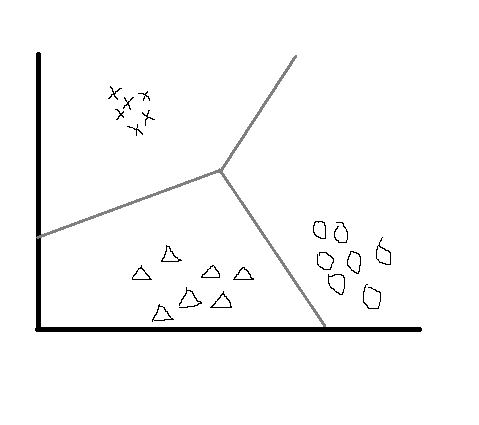
\includegraphics[scale=0.5]{billeder/oneofk1}
\caption{1-of-k linear classifier for 3 classes}
\label{oneofk1}
\end{figure}
In math terms the one-vs-one can be written as:
\begin{equation}
\label{oneofkcostfunc}
y(\textbf{x})=\tilde{\textbf{w}}^T\tilde{\textbf{x}}
\end{equation}
This is because we can consider the output y to be a weighted sum of the inputs. The error function can be defined as:
\begin{equation}
E(w) = \Sigma_n (\hat{y}(w,x_n) - y_n)^2
\end{equation}
Where $\hat{y}$ is the estimated $y$ value and $y_n$ is the true $y$ value.

If we look at a case with more than two classes, the linear classifier is prone to ambiguity. We know that the ambiguity issue can be avoid by using the form:
\begin{equation}
y_k(\textbf{x})=\textbf{w}_k^T\textbf{x}+\omega_{k0}
\end{equation}
and choosing the value of x to be a part of class k if $y_k(\textbf{x})>y_{m}(\textbf{x})$ for all $m \neq k$. This leads to decision boundaries corresponding to the 1-of-k classifier where the decision boundaries join together in the middle corresponding to the image in figure \ref{oneofk1}.

\textbf{Training:}\\
Training the one-of-k function requires the use of two vectors in matlab: $t \& Z$. t is vector of the correct classes while Z is a vector containing our features. In order to train the one-of-k classifier we use the following equation:
\begin{equation}
w^* = (Z^T Z)^{-1} Z^T t
\end{equation}
This results in the estimated weights for the classifier. To classify the data we use the cost function described earlier in equation \ref{oneofkcostfunc}.

In order to observe the boundaries in the project, the data must be 2 or 3 dimensional. This will require either the use of the PCA or fisher reduction methods explained in early sections. This leads to the image seen in figure \ref{2dimoneofk}.
\begin{figure}[H]
\centering
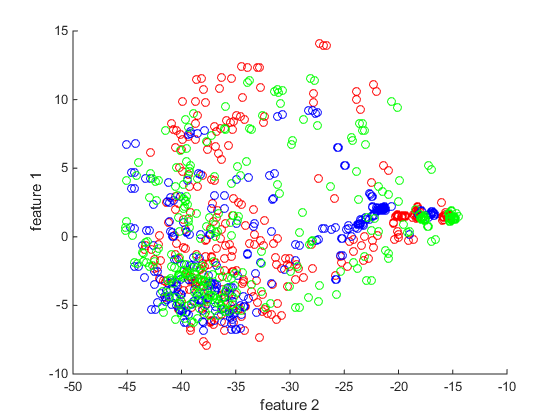
\includegraphics[scale=0.5]{billeder/2dimoneofk}
\caption{2 dimensional 1-of-k linear classifier for 3 classes of speech}
\label{2dimoneofk}
\end{figure}
This does not provide a usable visual representation of the classifier. The choice was made to keep the data in the higher dimensions. The output from the cost function provides a sample and the values representing the three classes:
\begin{verbatim}
0.5333
0.2506
0.2160
\end{verbatim}
The cost function classifies the first sample to belong to class 1 as an example.

\textbf{Intermediate results:}\\
The test data was split into 3 sections and run through the cost function. This resulted in three plots as can be seen in figure \ref{fig:oneofkval1}, \ref{fig:oneofkval2} \& \ref{fig:oneofkval3}. The classes are coloured: Nicolai = Red, Reimer = Blue, Rune = Green.
\begin{figure}[H]
\minipage{0.32\textwidth}
  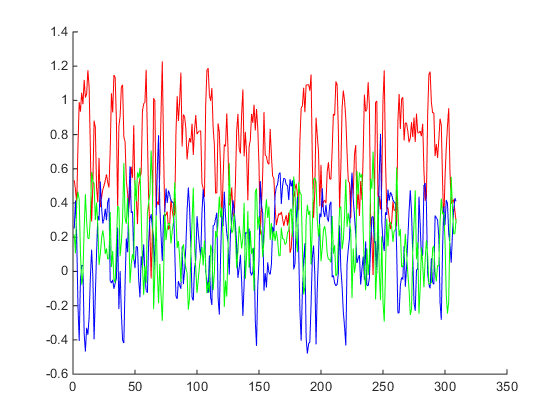
\includegraphics[width=\linewidth]{billeder/oneofkval1}
  \caption{Output from first 1/3 of the data}\label{fig:oneofkval1}
\endminipage\hfill
\minipage{0.32\textwidth}
  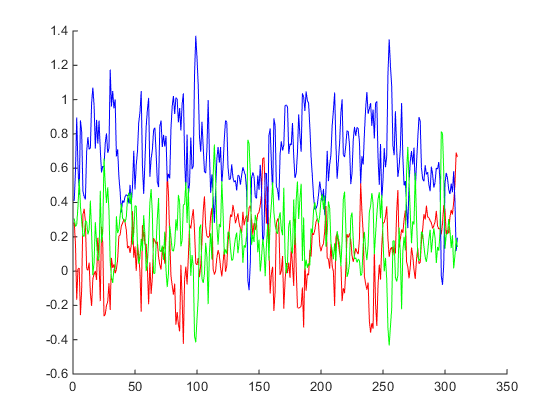
\includegraphics[width=\linewidth]{billeder/oneofkval2}
  \caption{Output from middle 1/3 of the data}\label{fig:oneofkval2}
\endminipage\hfill
\minipage{0.32\textwidth}%
  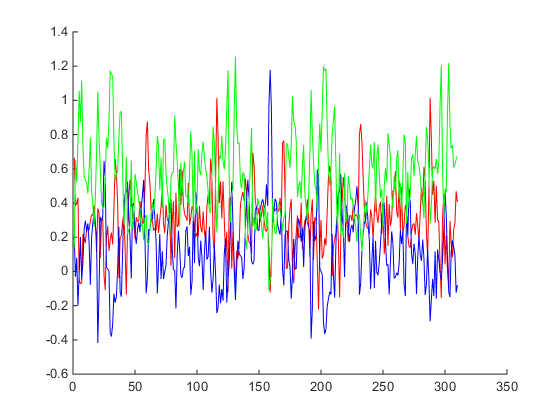
\includegraphics[width=\linewidth]{billeder/oneofkval3}
  \caption{Output from last 1/3 of the data}\label{fig:oneofkval3}
\endminipage
\end{figure}
When evaluating the peak values of the three plots, it can be observed that the first 1/3 of the data belongs to class 1, the middle 1/3 of the data belongs to class 2 and the rest of the data belongs to class 3.

%------------------------------------------------
\subsection{Probabilistic models}
In many cases the features follows a certain distribution. By using the information in the distribution it is possible to filter out outliers and determine how likely it is that the point belongs to a certain class. This can be very powerful since we not blindly put a sample in a class but also get information about the likelihood. This of course demands that a qualified guess of the distribution can be made. 
By using the probability for a given sample, given a certain class $P(x|C)$. Iteration over the the different classes, it is possible to decide were to classify the sample, and how certain we are of this decision. This is illustrated in figure X. 
\fxnote{(fix me) figure 2}



\subsubsection{Discriminative Model}

Instead of asking what the probability of the sample, given the class is $P(x|C)$, the conditional probability can be used. That is the probability of a class, given a sample $P(C|x)$. This can be found using Bayes rule:
\begin{equation}
 P(C|x)=\frac{P(x|C)P(C)}{P(x)}
\end{equation}
This kind of model is called a discriminative model, and is used for modelling the dependence of an unobserved class $C$ on an observed variable $x$. This will for the Gaussian distribution be a sigmoid function. Using this model to classify it is no longer able to tell about the probability of a sample not being in any class, but on the same time also simplifies the classifier a lot. Compared to the linear classifier the discriminative classifier are able to create a mouth sharper decision bound. If the sharper decision bound is the goal then a easer approach is to estimate the optimal sigmoid for separation of classes directly. This can be done by optimizing a soft-max function to separate the classes. The soft-max function is expressed as: 
\begin{equation}
\label{eq:softmax}
 Y_k(w_k,x)=\frac{e^{w_k x}}{\sum\limits_{k=1}^K e^{w_k x}}
\end{equation}
Comparing this to the previous probabilist function we can assume that:
\begin{equation}
\label{eq:baseassmution}
 P(t|w,x) = p_n^t (1-p_n)^{1-t} , t \in [0,1] 
\end{equation}
Here we see how likely it is that the class vector t, is correct given data point x, and some weights w in the soft-max.  Where t is the class vector, that indicates which class the data point x is part of.  The $p_n$ is given by: 
\begin{equation}
 p_n = P(C| w, x) = y(w,x)
\end{equation}
The challenge is now to find the optimal weights $w_k$, for each class, to create the best classifier. This can be done by combining the two equations \ref{eq:softmax}, \ref{eq:baseassmution} to create a non linear optimisation problem.
\begin{equation}
 L(w) = \log{\prod\limits_{i=1}^N y(w,x_i)^{t_i} ( 1-y(w,x_i))^{1-t_1}}
 = \sum\limits_{i=1}^N t_i\log{y(w,x_i)}+(1-t_i)\log({1-y(w,x_i))}
\end{equation}
This can be solved by many different optimizations strategies. By optimizing this for each class we will find the optimal weights for the soft-max class separator in equation \ref{eq:softmax}.\\

In the speaker recognition case a soft-max function has been used to create a discriminative model, that are able to separate the classes as described above. A full probabilistic model using the $P(x|C)$ approach, has also been attempted by using a Gaussian mixture model. This is described in the section: \ref{sec:EMGMM}. In this analysis it is assumed that the data is Gaussian distributed. This assumption is made by looking at the histogram of the features. This is shown on figure ( fix me).\\

show figure 1\\

By running the optimizing the soft-max function a model is found that are capable of separating the test set in the three classes, whit a 21.58 \% error rate. The results can be seen in table \ref{tab:resultTableProp}. 

\begin{table}[h]
\centering
\begin{tabular}{ll}
\hline
Total Error   & 21.58 \% \\ \hline
Nicolai Error & 24.27 \% \\
Rasmus Error  & 10.68 \% \\
Rune Error    & 29.77 \% \\ \hline
\end{tabular}
\caption{Discriminative Model Results}
\label{tab:resultTableProp}
\end{table}

The results indicate that Rune is the one there is hardest to classify. Even though some samples are classified wrong, the majority of samples is correct classified. This makes this method valid for speaker recognition. \\
\ \\

\fxnote{have awesome glud billed .}

%------------------------------------------------
\subsubsection{Gaussian Mixture Models}
\label{sec:GMM}
One of the most common distributions is the Gaussian distribution $ \mathcal{N}(\mu,\sigma)$. Sometimes this model is not quiet enough to capture the underlying distribution. In such cases can a mixture of Gaussian distributions be created to fit a underlying distribution. This principal is shown in figure \ref{fig:mixturemodel}. 

\begin{figure}[H]
\centering
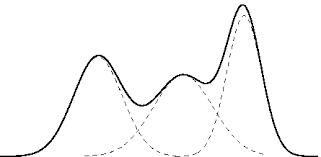
\includegraphics[scale=0.5]{billeder/MixtureModel}
\caption{Gaussian Mixture Model Principe}
\label{fig:mixturemodel}
\end{figure}

This method can be generalized up in a multidimensional space, to fit the feature space. In a multidimensional model we introduce the covariance matrix $\Sigma$ that like $\sigma$ gives the deviation of a Gaussian model. The Gaussian mixture model can therefore be described as: 

\begin{equation}
 P(x) = \sum\limits_{k=1}^K{ \Pi_k \mathcal{N}(x|\mu_k,\sigma_k) }
\label{eq:mixturemodel}
\end{equation}

Where $\Pi_k$ is a weight called the mixture parameter, that is used to differentiate the individual Gaussian distributions in the model. knowing this we can also describe the mixture model from equation \ref{eq:mixturemodel} as: 

\begin{equation}
 P(x) = \sum\limits_{k=1}^K{ P(k) P(x|k) }
\label{Eq:mixturemodel}
\end{equation}

In order to use a the mixture model, the different distributions must first be found. This topic will be discussed in section \ref{sec:k-means} and \ref{sec:EMAlgorithm}

\subsubsection{k-means Algorithm}
\label{sec:k-means}

One way of finding groupings of data, in the feature space, is by using the k-means algorithms. This algorithm tries to split the data in k groups. This is done by following 4 three step iterating proses. 

\begin{enumerate}
  \item Initialize means: Select k random mean values in the feature set. 
  \item Assign responsibility: For each point, find the closest mean points and make it responsible for that point.
  \label{step:iteratemeans} 
  \item Calculate new mean: Move each mean point to the mean value of the cluster of points the mean is responsible for. 
  \item Continue whit step \ref{step:iteratemeans}, till no change in points. 
\end{enumerate}

On figure \ref{fig:kmeans} is illustrated how the k-means in 6 iterations split the data up in 3 clusters.

\begin{figure}[H]
\centering
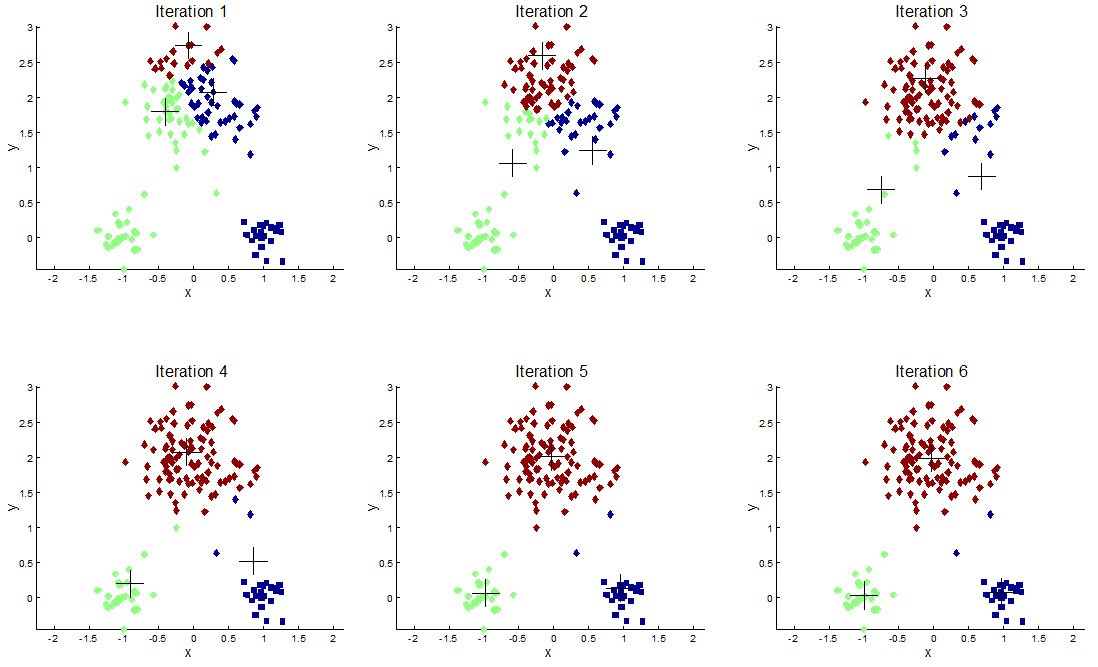
\includegraphics[scale=0.6]{billeder/kmeansclustering}
\caption{K-means used on a data set}
\label{fig:kmeans}
\end{figure}

The result of this proses will differ depending on the initial mean guesses. This is especially the case is there is no natural groupings in the dataset. In this case the algorithm will still split up the data in k clusters there are side by side. This is illustrated on figure \ref{fig:badkmeans}, where the k-means algorithm tries to cluster points distributed uniformly on a circle, in 7 clusters. 

\begin{figure}[H]
\centering
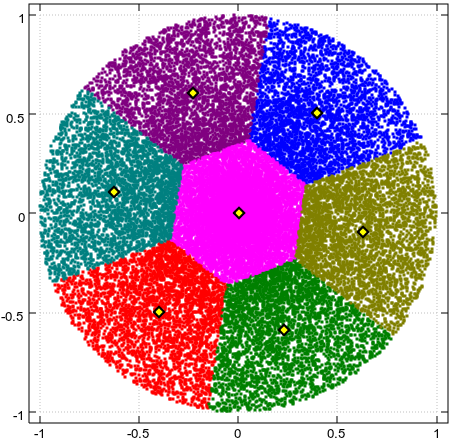
\includegraphics[scale=0.5]{billeder/CircleClusters}
\caption{K-means used on points distributed uniformly on a circle}
\label{fig:badkmeans}
\end{figure}

\subsubsection{EM Algorithm For Gaussian Mixture Models}
\label{sec:EMAlgorithm}

As discussed in section \ref{sec:GMM} it is important to have a method of finding the best Gaussian distributions in the data set to create a good mixture model. The best Gaussian Mixture Models that fits the data can be described as optimising equation \ref{eq:maxgmm}.

\begin{equation}
 L(x) = \sum\limits_{n=1}^N{\log{\sum\limits_{k}^K P(k) P(x_n|k) }}
\label{eq:maxgmm}
\end{equation}

To find the maximum of equation \ref{eq:maxgmm}, we find the differentiated and set et equal zero. 

 \begin{equation}
 \frac{\partial L(x)}{\partial{\mu_k}} = 0
\label{eq:partialzero}
\end{equation}

From equation \ref{eq:mixturemodel} and \ref{eq:partialzero} the following optimisations equations can be found: 

\begin{equation}
 N_k = \sum\limits_{k}^K P(k|x_n)
 \label{eq:em1}
\end{equation}
\begin{equation}
 P(k)= \Pi_k = \frac{N_k}{N}
 \label{eq:em2}
\end{equation}
\begin{equation}
 \Sigma_k= \frac{1}{N_k} \sum\limits_{n}^N{ P(k|x_n) (x_n -\mu_n)(x_n-\mu_k)^\intercal}
 \label{eq:em3}
\end{equation}
\begin{equation}
 \mu_k= \frac{1}{N_k} \sum\limits_{n}^N{ P(k|x_n) x_n}
 \label{eq:em4}
\end{equation}

The variable $N_k$ can be seen as the effective number of samples in a cluster, and $N$ is the total number of samples. The $P(k|x_n)$ term can be seen as the responsibility a center point has for that point. Unlike the K-means algorithm the all center points are responsible for all points, but the level of responsibility is different from center point to center point. To find the optimal center points $\mu_k$, and there deviations $\Sigma_k$ the EM algorithm can be used. This is based on a the idea of a E-step, called the estimation step, and a M-step called the maximisation step. Much like the k-means does this also have 4 iterative steps. 


\begin{enumerate}
  \item Initialize Parameters: Select k random values for $\mu_k$ , $\Sigma_k$ , $\Pi_k$
  \item E-Step: Update the responsibility by using Bayes' theorem stating: 
 \begin{equation}
 	P(k|x) = \frac{P(x|k) P(k)}{P(x)} = \frac{P(x|k) P(k)}{\sum\limits_{k}^K{ P(x|k) P(k)}}
 \end{equation}
  
  \item M-Step: Maximize the Gaussian mixture model parameters by using equations \ref{eq:em1}, \ref{eq:em2}, \ref{eq:em3} and \ref{eq:em4}. 
  
  \item Continue whit step 2, till no change in Gaussian mixture model parameters. 
\end{enumerate}

Like the k-means algorithm does this algorithm also map a predetermined number of Gaussian distributions to the dataset. The optimal amount must be found though exploration. On figure \ref{fig:UGMM} we see how the EM algorithm has been used to map 3 Gaussian mixture model to a dataset. 

\begin{figure}[H]
\centering
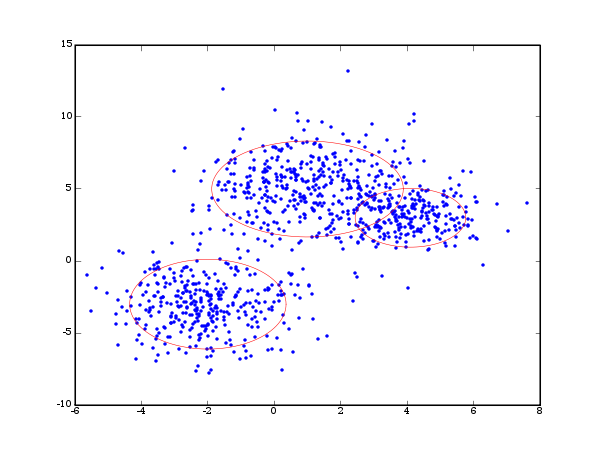
\includegraphics[scale=0.5]{billeder/UGMM}
\caption{EM Algorithm Used On Data To Create GMM}
\label{fig:UGMM}
\end{figure}

Like for the k-means the initial start estimates for the mean value is important for a good result, and a fast execution time. A normal approach is to use the k-means algorithm first, and use the final means as the start estimate in the em algorithm. In order to reduce the training time, the model is sometimes reduced in complicity. Instead of a full Gaussian distribution a spherical covariance or a completely diagonal covariance is used. 

\subsubsection{Unsupervised Gaussian Mixture Model}
Sometimes the training data is unlabelled, which mean that the classes is unknown. In such data there can still be some underlying structures, that can be used to classify the data. The goal of unsupervised learning is to discover these structures, and create the classes from them. \\ \ \\
One approach of this is to select a number of desired classes, and try finding clusters in the data to fit to the classes. This can be done whit the k-means as shown in figure \ref{fig:kmeans}.  where 3 classes is found to fit the data. Likewise can the Gaussian mixture model also be used to find distributions that describes the classes. This can be seen in figure \ref{fig:UGMM} where 3 Gaussian distributions is fit to the unlabelled data. \\ \ \\

In the speech recognition case we have investigated if it is possible to use the Gaussian mixture model as a unsupervised method to find the 3 persons: Nicolai, Rasmus and Rune. For this to work the features must be placed in separated clusters corresponding to the persons. 

When evaluating this we see that the classes found does not correspond to the 3 know classes. The when looking at the errors on table \ref{tab:resultTableUGMM}, it is seen how the error for every one over 50%. 


\begin{table}[H]
\centering
\begin{tabular}{ll}
\hline
Total Error   & 65.24 \% \\ \hline
Nicolai Error & 53.10 \% \\
Rasmus Error  & 78.34 \% \\
Rune Error    & 64.27 \% \\ \hline
\end{tabular}
\caption{Unsupervised GMM Results}
\label{tab:resultTableUGMM}
\end{table}
 
This means that this method is not able to automatically split the data up in the desired classes.
 
\subsubsection{Supervised Gaussian mixture model}
\label{sec:EMGMM}

What if we used the same method to train the data, but in a supervised manner. A other method is to train a Gaussian mixture model for each class, and use this to classify. A Gaussian mixture model was trained to each voices. To find the optimal amount of Gaussian distributions was a experiment where we started at one and ended whit 10.

\begin{figure}[H]
\centering
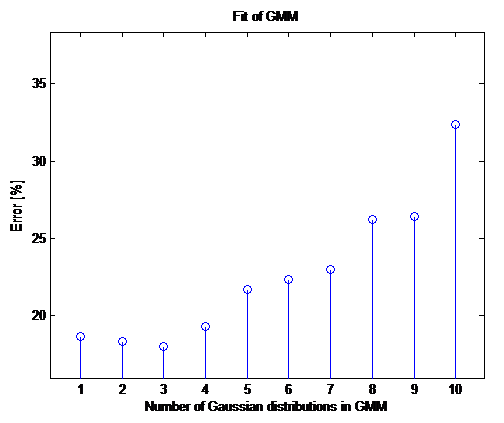
\includegraphics[scale=0.7]{billeder/fitGmm}
\caption{GMM fit in relation to number of Gaussian distributions}
\label{fig:fitGMM}
\end{figure}

As seen on figure \ref{fig:fitGMM}, three Gaussian distributions in each GMM is the one that gives the lowest error. To ensure that 18\% is the best we can achieve whit this model, the model is retrained whit random initializations. The best fit found whit this configuration can be seen in table \ref{tab:resultTableSGMM}.

\begin{table}[H]
\centering
\begin{tabular}{ll}
\hline
Total Error   & 15.64 \% \\ \hline
Nicolai Error & 9.06 \% \\
Rasmus Error  & 21.68 \% \\
Rune Error    & 16.18 \% \\ \hline
\end{tabular}
\caption{Supervised GMM Results}
\label{tab:resultTableSGMM}
\end{table}

Here it is seen how this model is relative good at separating the data in the  the three classes. This model have the most trouble finding Rasmus, this is noticeable different from the other models where Rune is the hardest to recognize. 

%------------------------------------------------
\subsection{Artificial Neural Network Classifier}

\lettrine[nindent=0em,lines=3]{L} orem ipsum dolor sit amet, consectetur adipiscing elit.
\lipsum[2-3] % Dummy text

\lettrine[nindent=0em,lines=3]{L} orem ipsum dolor sit amet, consectetur adipiscing elit.
\lipsum[2-3] % Dummy text}

\lettrine[nindent=0em,lines=3]{L} orem ipsum dolor sit amet, consectetur adipiscing elit.
\lipsum[2-3] % Dummy text

%------------------------------------------------
\subsection{Sequential Models}
Markov model and Hidden Markov Model.

e.g. meaning of parameters, left-to-right model, outline of training/testing method.\\

Introtext\\

Math\\

How we use it or why we don't use it\\

Intermediate result\\\ \\

%------------------------------------------------

The classifiers presented until this point have been stateless. This means that each point is being classified solely on its values, and not in the context of samples. But sometimes information about how the features change over time can be used to determine the class. An example of this is in word recognition, where the order the letters come in is important for recognizing a word.  If we look at the following two words:

\begin{itemize}
  \item "Cow"
  \item "Coooww"
\end{itemize}

It is easy to see that it is the same word, some of the letters is just repeated in the second case. This is often the case when trying to recognize words in speech, due to the variance in speed from person to person. To model this we could look for the probability of: 

\begin{equation}
 P(x_1, x_2, ..., x_5) = P(x_5| x_4,x_3,x_2, x_1) P(x_4| x_3,x_2, x_1) P(x_3|x_2, x_1) P(x_2|x_1) P(x_1)
 \label{eq:seqmodel}
\end{equation}

Which simply states that the probability of a given sequence, is the probability of the first letter multiplied by the probability of the next letter, given the first, and so on. To model this kind of behavior a Markov model can be used.

\subsubsection{Markov Model}
The Markov model is a way of modelling a sequential dependency in the data. Much like before does the data need to be spilt into classes, called states. The The Markov model does not deal whit splitting the data into states, but rather in what order the data transitions between states.\\\ \\

In the Markov model it is assumed that the state only is determined by the last sample. Mathematically described as shown in equation \ref{eq:markovpremis}.

\begin{equation}
 P(x| x_{n-1}, x_{n-2}, ..., x_1) = P(x| x_{n-1}) 
 \label{eq:markovpremis}
\end{equation}

This assumption simplifies equation \ref{eq:seqmodel}, so we know have:

\begin{equation}
 P(x_1, x_2, ..., x_n) = P(x_1) \prod\limits_{n=2}^N{P(x_n| x_{n-1})}
\end{equation}

This is also called a Markov chain or a first order Markov model, since it is only depended on the last sample. Variations of the model does exists that takes more than just the last sample in consideration, but will not be further discussed in this report.  
\\\ \\
A simple Markov model is shown in figure \ref{fig:simpleMarkov}. This is a illustration of the previous "Cow" example, where each letter is a state. Here we assume that we always start in state "C". From here we have 95\% chance of moving to the "O" state and 5\% chance of staying in the "O" state. 

\begin{figure}[H]
\centering
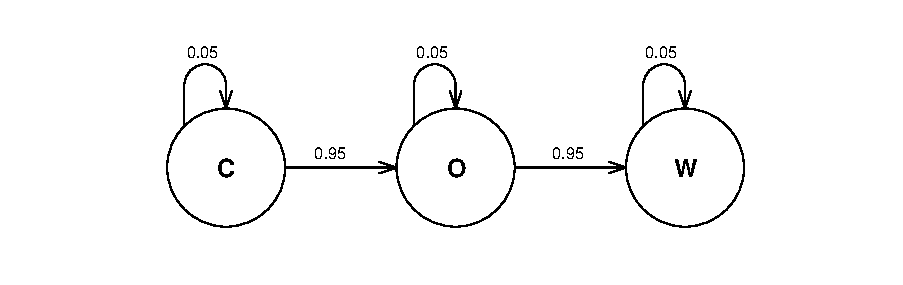
\includegraphics[scale=0.8]{billeder/simpleMarkov}
\caption{Markov model for the word "COW"}
\label{fig:simpleMarkov}
\end{figure}
		
In this model there is 0\% chance of moving from state "C" to "W". It is only possible to go to the same state, or change to the next in the letter series. This kind of model is called a Left-to-right model. This model is often used in this kind off application, but for other applications a other model where it is possible to jump between many states could be relevant. The states transaction is often given in a transaction matrix: 
\begin{equation}
	A_{n,n-1} = 
	\begin{bmatrix}
  	0.05 & 0.95 & 0 \\
  	0 & 0.05 & 0.95	\\
  	0 & 0 & 	1
 	\end{bmatrix}
 	\label{eq:Amat}
\end{equation}

In equation \ref{eq:Amat} the transition matrix is shown for the word "COW" illustrated by the transition graph in figure \ref{fig:simpleMarkov}. The matrix is an $M\times M$ matrix, where $M$ is the number of states. Each row and column is symbolizing the states, and the cells contains the transition probability from a row element to a column element.


\subsubsection{Hidden Markov Model}
A hidden Markov model is a Markov model in which the system being modelled is assumed to be a Markov process with unobserved states, also known as hidden states. It also have a set of desired output states. Like for the normal Markov model there is a transition between the hidden states given by a transition matrix $A$. For each hidden state there is also a probability of a given output state this is called the emission probability.

\begin{figure}[H]
\centering
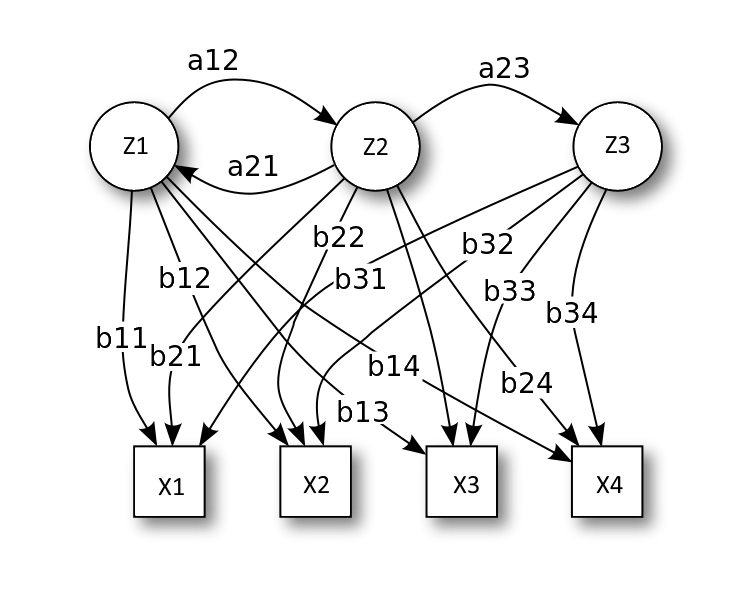
\includegraphics[scale=0.5]{billeder/HiddenMarkovModel}
\caption{Hidden Markov Model}
\label{fig:HiddenMarkov}
\end{figure}

This is illustrated on figure \ref{fig:HiddenMarkov}, where x is the known output states. The z is the hidden input states and a is the transaction parameters and b is the emission parameters. the probability for a given hidden sequence and output can be described as: 
\begin{equation}
 P(x_1, ..., x_n, z_1, ..., z_n) = P(z_1) \prod\limits_{n=2}^N{P(z_n| z_{n-1})} 
\prod\limits_{n=1}^N{P(z_n| z_n)}
\end{equation}
 
For many applications we do not know the hidden state of the data, but only the desired output state. It is therefore desired to make a training session that finds the optimal hidden states, and transition and emission parameters that gives us the best fit to the desired output states. 


%!TEX root = ..\Master.tex

\subsection{Support Vector Machines}
The support vector machine is a supervised learning algorithm.
Compared to neural network, it sometimes gives a cleaner and more powerful way of learning complex non-linear functions. (TODO: What does more powerful mean?)

\subsubsection{Linear}
When doing the linear classifier, SVM will try to find the line that seperates the data with the highest margin as seen on figure \ref{fig:svm-margin}.

\begin{figure}[H]
\centering
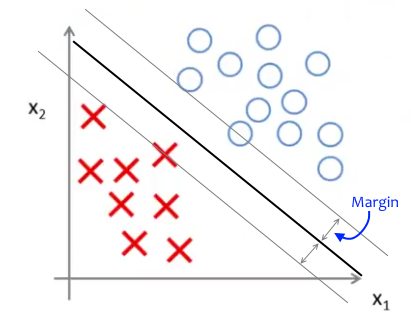
\includegraphics[scale=.75]{billeder/svm-margin}
\caption{Large margin classification.}
\label{fig:svm-margin}
\end{figure}

By solving the optimization problem defined as equation \ref{eq:svm-linear-optimization}, we find the parameters for the linear SVM classifier.
\begin{equation}
\min_{\theta}C \sum_{i=1}^{m}
\left[ y^{(i)}cost_1(\theta^Tx^{(i)})+(1-y^{(i)})cost_0(\theta^Tx^{(i)}) \right]
+ \frac{1}{2}\sum_{i=1}^{n}\theta^2_j
\label{eq:svm-linear-optimization}
\end{equation}
We must choose the value of the constant $C$. (TODO: what is its effect? Some regularization thing.)
Figure \ref{fig:svm-cost-function} shows the plot of $cost_0$ and $cost_1$.
\begin{figure}[H]
\centering
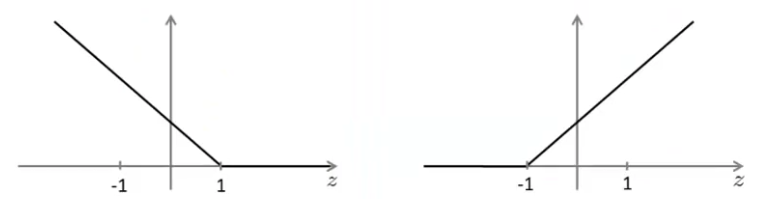
\includegraphics[scale=.75]{billeder/svm-cost-function}
\caption{Left: $cost_1(\theta^Tx^{(i)})$. Right: $cost_0(\theta^Tx^{(i)})$}
\label{fig:svm-cost-function}
\end{figure}

Hypothesis: (TODO: Is this correct? shouldn't it be 1 if $\theta^Tx \geq 1$ and 0 if $\theta^Tx \leq -1$)
\begin{equation}
h = 
\begin{cases}
1 & \text{if}\ \theta^Tx \geq 0 \\
0 & \text{otherwise}
\end{cases}
\end{equation}

\subsubsection{Non-linear}
Finds the kernels that seperates the data best.
gaussian kernels.

\begin{figure}[H]
\centering
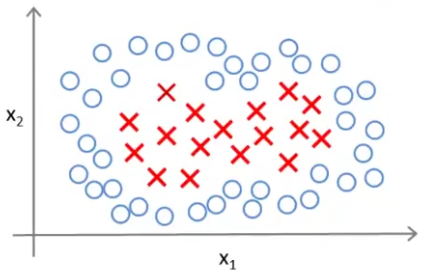
\includegraphics[scale=.75]{billeder/svm-non-linear}
\caption{Example of problem that requires non-linear classification.}
\label{fig:svm-non-linear}
\end{figure}

The gaussian kernel function:
\begin{equation}
f_i = similarity(x,l^{(i)}) =
exp\left(-\frac{||x-l^{(i)}||^2}{2\sigma^2}\right)
\end{equation}

At each training example we will put a landmark:
\begin{equation}
\begin{split}
\text{Given}\ (x^{(1)},y^{(1)}),(x^{(2)},y^{(2)}),\dots,(x^{(m)},y^{(m)}),\\
\text{choose}\ l^{(1)} = x^{(1)},l^{(2)} = x^{(2)},\dots,l^{(m)} = x^{(m)}
\end{split}
\end{equation}

We convert the training data into new feature vectors. For training example $(x^{(i)},y^{(i)})$:
\begin{equation}
f^{(i)}=
\begin{bmatrix}
f_0^{(i)} \\
f_1^{(i)} \\
\vdots \\
f_m^{(i)}
\end{bmatrix}
\end{equation}
 where $f_0^{(i)} = 1$.

The minimization problem now looks like:
\begin{equation}
\min_{\theta}C \sum_{i=1}^{m}
\left[ y^{(i)}cost_1(\theta^Tf^{(i)})+(1-y^{(i)})cost_0(\theta^Tf^{(i)}) \right]
+ \frac{1}{2}\sum_{i=1}^{m}\theta^2_j
\end{equation}

A large C gives lower bias and high variance, which means it uses a smaller amount of regularization and is more prone to overfitting. \\
A small C gives higher bias and low variance, which means it uses a higher amount of regularization and is more prone to underfitting. \\
A large $\sigma^2$ gives higher bias and lower variance, which means that features $f_i$ varies more smoothly. \\
A small $\sigma^2$ gives lower bias and higher variance, which means that features $f_i$ varies less smoothly.

In this project the softmax SVM is used with the constraint being:
\begin{equation}
w^* = ARG MIN (||w||^* + C \sum \epsilon_n)
\end{equation}
Inputting the features from this project along with a vector \textbf{t} that describes which class the features belong to.


%------------------------------------------------
\section{Results}

All the methods have been compared against each other. In the comparison all method have been in a "must classify" setting. This means that each sample is put in a class, even though the probabilistic method says that the odds of it belonging in any class is very little. Each sample can also only belong to one class, and we be assigned to the class with the highest probability. For these test the data was split so 70\% was used as training and the remaining 30\% to validation. Further more was the amount of samples normalized, so each class had the same amount of training and test samples.


\begin{table}[H]
\centering
\begin{tabular}{llllll}
\hline
Class		&	Linear	&  Discriminative  & GMM  & ANN	& SVM \\ \hline
Nicolai Error &	24.91\%  & 24.27\%  &  9.06\%  & 10.35\%  &  3.56\% \\
Rasmus Error  &	11.00\%  & 10.68\%  & 21.68\%  & 10.03\%  & 24.92\% \\
Rune Error	  &	30.74\%  & 29.77\%  & 16.18\%  & 16.82\%  & 36.57\% \\ \hline
Total Error	  &	22.22\%  & 21.58\%  & 15.64\%  & 12.41\%  & 21.68\% \\ \hline
\end{tabular}
\caption{ Error of test data }
\label{tab:restest}
\end{table}

On table \ref{tab:restest} it is shown how many percent error that was in each class, and the total error of all classes, when classifying the test data, with the different methods. Even though this is the most important metric of validation, it can be interesting to see how well it classifies to 70\% training data. This is shown in figure \ref{tab:restrain}, where the error as expected is way lower.

\begin{table}[H]
\centering
\begin{tabular}{llllll}
\hline
Class		&	Linear	&  Discriminative  & GMM  & ANN	& SVM \\ \hline
Nicolai Error &	14.76\%  & 10.34\%  &  0.41\%  & 0\%  &  0\% \\
Rasmus Error  &	10.48\%  & 11.59\%  & 0.14\%  & 0\%  & 0\% \\
Rune Error	  &	23.17\%  & 18.48\%  & 2.06\%  & 0\%  & 0\% \\ \hline
Total Error	  &	16.14\%  & 13.47\%  & 0.87\%  & 0\%  & 0\% \\ \hline
\end{tabular}
\caption{ Error of training data }
\label{tab:restrain}
\end{table}

But the tables does not supply any information about the distribution of the errors. In order to validate that the method can be used for classification, is a experiment done where the algorithms have to separate a sound file in who's talking when. The sound file is first Nicolai talking then Rasmus and in the end Rune. Each person talks in the same amount of time, and no one is talking on the same time.  After classifying all samples, is a 20 tab median filter used to determine who is talking. The results can be seen in figure \ref{fig:talktest}. 

\begin{figure}[H]
\centering
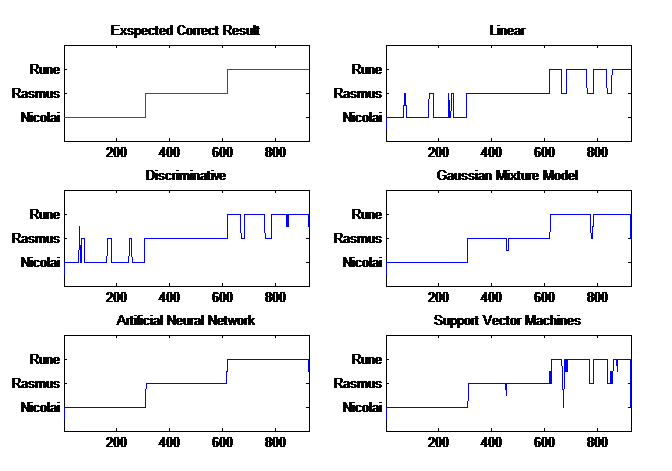
\includegraphics[scale=0.9]{billeder/TestedMethods}
\caption{ Find who is talking }
\label{fig:talktest}
\end{figure}

All mesurements in tabel \ref{tab:restest} and \ref{tab:restrain} have been done with a PCA reduction to 40 features. To investigates the PCA reduction effect on the different methods a series of measurements was done. In this series there was started by reducing to one feature and increasing the number of features until 60 was reached. The result of this test can be seen in figure \ref{fig:DimError}.

\begin{figure}[H]
\centering
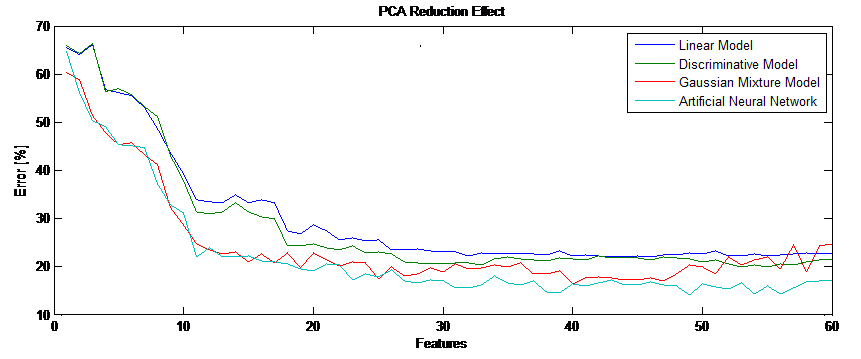
\includegraphics[scale=0.7]{billeder/PCAReductionEffect}
\caption{ Dimensions effect on Error }
\label{fig:DimError}
\end{figure}

%------------------------------------------------

\section{Discussion}
When looking at the results from table \ref{tab:restest}, it is easy to see that the linear methods: Linear classifier and support vector machines, is worse than the probabilistic methods. This is often the case if the classes is not clusterable, which make it hard to draw a good decision bound. The probabilistic methods is quite good in comparison, and the best match is archived by using the artificial neural network method, which only have a 12.41\% error. \\\ \\

Looking at how well the methods was able to classify the training data, as shown in figure \ref{tab:restrain}. It is seen that the support vector machine and the artificial neural network is capable of classifying the data perfectly whit no error. This is often a indication of over fitting, and you must therefore be very cautious whit the results. By making a extensive search in the solution set of these two methods, we found that this was also the best classifier of the test data, which tells us that over fitting was not the case. Instead this is a result of a very small test set, that makes it possible to completely satisfy the training scenario. This makes the classifiers very specialized. \\\ \\


When looking how the different classifiers perform on the different classes, it is shown that Rune is the one that is generally hardest to recognize. Only in the supervised Gaussian mixture model is this different where Rasmus is the hardest.  It is also seen that for the linear and Discriminative classifier, Rasmus is the easiest to find, but for the other models it is Nicolai. \\\ \\

All the presented methods in table \ref{tab:restest} is able to do classification of a speaker, since there are way more correct guesses than wrong. This can also be seen in figure \ref{fig:talktest}. It is also easy to see from this figure that support vector machines only struggle to classify Rune, but have no problem whit Nicolai and Rasmus. Figure \ref{tab:restest} also shows that the errors for the neural network is not happening in bursts, and is therefore filtered out \\\ \\

Looking at the PCA reduction in figure \ref{fig:DimError} it is seen how the error rate seems to stabilize at 30 features, regardless of algorithm used.


\section{Conclusion}
Using the a MFCC transformation of the audio data, we ware able to get some representative features fore who is speaking. The classification was also tried on features only extracted from the frequency using a FFT. But the MFCC features was way superior to these, so in order to get the simplest model, the FFT features was removed. \\\ \\

In order to further simplify the model, was dimensionality reduction used. Two method of dimensionality reduction was tried PCA and the Fisher method. Even though Fisher theoretically gives the best separation between the classes, does it have the limitation of only reducing to k-1 features. Since we in this project only have three classes, this means we max can get two features. This turns out to be too few classes to do a good classification. Using the PCA reduction to is found that more than 30 PCA reduced features gives the best classification.  \\\ \\ 

In the project have a range of linear, probabilistic and sequential models been used to create a speaker recognition system. It is found that due to the lag of sequential dependency in the features, is the sequential model not suitable for this kind of application. Where the linear and probabilistic models all yields good results. The worst classifier found is the linear classifier that 22.22\% error. Event though this is the one that preforms the worst, it is also the most simple to train and use. The best classifier found was the artificial neural network which only have an error rate on 12.41\%. Compared to the linear classifier is this a very hard to train, but is relative easy to use, when trained. \\\ \\  

When looking at the test result it is clear that the fairly small dataset have had a impact on the performance, and for training a similar application for commercial use way more data is needed. 


\listoffixmes

%----------------------------------------------------------------------------------------
%	REFERENCE LIST
%----------------------------------------------------------------------------------------
\begingroup
	\raggedright
	\bibliography{bibtex/litteratur}							% Litteraturlisten inkluderes
\endgroup

%----------------------------------------------------------------------------------------

%\end{multicols}

\end{document}